\documentclass[doc, floatsintext]{apa7}
\usepackage[style=apa,sortcites=true,sorting=nyt,backend=biber]{biblatex}
\DeclareLanguageMapping{american}{american-apa}
\addbibresource{sample.bib}
\setlength\bibhang{.15in}
\usepackage{amsmath}
\usepackage{float}
\usepackage{graphicx}
\usepackage{mathrsfs}
\usepackage{setspace}
\setstretch{1.0}
\usepackage{caption}
\usepackage{gensymb}

\title{Criterial Learning and Feedback Delay: Insights from
Computational Models and Behavioral Experiments}
\shorttitle{Computational Criterion Learning}

\authorsnames[{1, 2}, {3}, {4}]{
    Matthew J. Crossley, 
    Benjamin O. Pelzer,
    F. Gregory Ashby
}

\authorsaffiliations{
    {School of Psychological Sciences, Macquarie University, Sydney, Australia}, 
    {Macquarie University Performance and Expertise Research Centre, Macquarie University, Sydney, Australia},
    {Nanyang Technological University},
    {Department of Psychological \& Brain Sciences, University of California, Santa Barbara}
    }
\abstract{The notion of a response criterion is ubiquitous
    in psychology, yet its cognitive and neural
    underpinnings remain poorly understood. To address this
    shortcoming, three computational models that capture
    different hypotheses about criterial learning were
    developed and tested. The time-dependent drift model
    assumes the criterion is stored in working memory and
    that its value drifts over time. The delay-sensitive
    learning model assumes that the magnitude of criterial
    learning is temporally discounted by feedback delay. The
    reinforcement-learning model assumes that criterial
    learning emerges from stimulus-response association
    learning without an explicit representation of the
    criterion, with learning rate also temporally discounted
    by feedback delay. The performance of these models was
    investigated under varying feedback delay and intertrial
    interval (ITI) durations. The time-dependent drift model
    predicted that long ITIs and feedback delays both impair
    criterial learning. In contrast, the delay-sensitive and
    reinforcement-learning models predicted impairments only
    with feedback delays. Two behavioral experiments, which
    tested these predictions, showed that human criterial
    learning is impaired by delayed feedback but not by long
    ITIs.  These results support the delay-sensitive and
    reinforcement-learning models, and suggest that even in
    tasks that appear to rely on explicit, rule-based
    reasoning, criterial learning may have strong
    associative underpinnings.
}

\authornote{Correspondence: Matthew J. Crossley, PhD,
  School of Psychological Sciences, Macquarie University,
  Australian Hearing Hub, 16 University Ave, Macquarie
  University, NSW 2109, Australia. Email:
  matthew.crossley@mq.edu.au 
}

\keywords{response criterion; criterial learning;
associative learning; categorization; procedural learning}

\begin{document}
\maketitle 

\section{Introduction}
The notion of a response criterion is ubiquitous in
psychology. It is a key component of almost all decision
models. For example, the hypothesis that even YES-NO
detection decisions are determined by comparing the sensory
magnitude to a response criterion that is under the
observer's control, rather than to a fixed absolute
threshold, allowed signal detection theory to supplant
classical threshold theory as the dominant model in
psychophysics \parencite{GreenSwets1966}. All models that
include a response criterion assume its value is learned and
can shift if changes are made to instructions or payoffs. So
criterial learning is a fundamental component of almost all
decision-making models. Despite its importance, however, the
cognitive and neural mechanisms that underlie criterial
learning remain poorly understood.

This article addresses this shortcoming through a
combination of computational modeling and empirical data
collection. Specifically, we develop and test three
different computational models that make qualitatively
different assumptions about how the criterion is learned.
The models differ in the role they assign to working memory
and in whether they treat the response criterion as a
fundamental psychological construct, or instead assume that
behavior is driven purely by stimulus-response associations
without any criterion guiding responses. These models are
then tested in two behavioral experiments. The modeling and
empirical focus are on how feedback delays and the length of
the intertrial interval (ITI) affect criterial learning. All
criterial-learning models assume that updating (i.e.,
learning) of the criterion occurs during the time interval
between feedback presentation and the stimulus presentation
that defines the onset of the next trial. So feedback delay
and the length of the ITI are the independent variables that
most clearly differentiate the conflicting predictions of
criterial-learning models. Furthermore, feedback delays are
known to impair some forms of learning (i.e., procedural)
much more than others (i.e., learning that relies on
declarative memory), so feedback-delay manipulations offer a
powerful method of disambiguating the nature of criterial
learning \parencite{ell2009critrial, MaddoxAshbyBohil2003,
MaddoxIng2005}.

Although the models could be tested in any task that depends
on criterial learning, the two experiments we describe used
a one-dimensional category-learning task. In such tasks,
stimuli vary across trials on two or more dimensions -- one
relevant to categorization and one or more that are
irrelevant. The observer's goal is to identify the relevant
dimension and learn the response criterion that maximizes
accuracy. This task has been used in hundreds of studies,
and all current models of performance in this task emphasize
the role of criterial learning.

In the first behavioral experiment, participants were
explicitly instructed about the relevant dimension, thereby
isolating criterial learning from rule selection and
switching processes. The results showed that short feedback
delays impaired learning compared to immediate feedback.
The second behavioural experiment used stimuli composed of
binary features -- where no criterial learning is needed --
and did not instruct participants about the relevant
dimension. Thus, this experiment isolated rule selection and
switching from criterial learning. The results found that
increasing feedback delay or ITI did not affect performance.
These findings suggest that feedback delays impact criterial
learning but not the discovery of the relevant stimulus
dimension.  More broadly, they indicate that criterial
learning may recruit procedural learning, even in tasks that
seem to rely on explicit, rule-based processes.

\section{Experiment 1: The Models}
We developed three computational models, each representing
different architectures of criterial learning, and examined
their sensitivity to the duration of ITIs and feedback
delay. Two of the models assume that the criterion is stored
in memory and that response decisions are made by comparing
the current stimulus-driven percept to this stored referent.
Both of these models further posit that the internal
representation of the criterion is updated following errors
using a simple gradient-descent rule. The third model
assumes that no criterion is stored nor used to generate
responses. Instead, reinforcement learning is used to form
stimulus-response associations and these associations drive
responding without any appeal to the notion of a criterion. 

For each of the three models, denote the time of stimulus
presentation on the current trial by T$_\text{S}$, the
response time by T$_\text{R}$, the time when feedback is
displayed by T$_\text{F}$, and the time when the stimulus
that begins the next trial is displayed by T$_{\text{S}^+}$.
Then note that the feedback delay equals
$\text{t}_\text{FD} = \text{T}_\text{F} - \text{T}_\text{R}$
and the duration of the ITI equals $\text{t}_\text{ITI} =
\text{T}_{\text{S}^+} - \text{T}_\text{F}$.

\subsection{Time-Dependent Drift Model}
The time-dependent drift model assumes that the observer
constructs a criterion, holds this value in working memory,
and then makes response decisions by comparing the percept
to the criterion. The model also assumes that both the
memory representation of the criterion and the perceived
value of the stimulus gradually drift over time. The model
further assumes that the extent of this drift increases with
time, both within a trial and between consecutive trials.

Let $x_n(t)$ and $c_n(t)$ denote the values of the percept
and the criterion, respectively, on trial $n$ at time $t$.
Then the decision rule on trial $n$ is:
\begin{equation}
  \text{Respond } R_n =
  \begin{cases}
    \text{A}, & \text{if ~} x_n(\text{T}_\text{S}) \leq c_n(\text{T}_\text{S})  \\
    \text{B}, & \text{if ~} x_n(\text{T}_\text{S}) > c_n(\text{T}_\text{S}).
  \end{cases}
  \label{eq:DR}
\end{equation}
If positive feedback is received, then the value of the
criterion remains unchanged for the next trial (except for
drift -- see Equation 3). If negative feedback is received,
then the criterion is modified according to the standard
model \parencite{SuttonBarto1998}:
\begin{equation}
c_n(\text{T}_\text{F}+ \Delta_t) = c_n(\text{T}_\text{F}) + \alpha [x_n(\text{T}_\text{F}) - c_n(\text{T}_\text{F})],
\label{RL}
\end{equation}
where $\alpha$ is a learning-rate parameter, and $\Delta_t$
is the time it takes to complete the updating. It is
straightforward to show that the iterative Equation \ref{RL}
is equivalent to computing a weighted mean (weighted by
recency) of the values of all percepts that occur on error
trials \parencite[e.g.,][]{Ashby2017}. This updating rule
will gradually converge on the optimal criterion value.
Since this model assumes that criterial learning relies on
working memory -- and the available evidence suggests that
logical reasoning and working memory are unaffected by
feedback delays of several seconds \parencite[e.g., in
one-dimensional rule-based category learning
tasks;][]{ell2009critrial, MaddoxAshbyBohil2003,
MaddoxIng2005} -- we assume that the learning process
described in Equation \ref{RL} is likewise unaffected by
feedback delay.

Although the criterial-learning process described by
Equation \ref{RL} is not affected by feedback delay, we
assume that both the stimulus and the criterion
representations drift randomly throughout the duration of
time they are maintained in working memory. The
representation of the criterion must always be maintained in
working memory, whereas drift in the stimulus representation
affects performance up until the feedback is presented, but
not afterwards.

We modeled the drift in both the criterion and the percept
by adding white noise to their initial values. Specifically,
we assumed that for all $t>\text{T}_\text{S}$
\begin{equation}
  c_n(t) = c_n(\text{T}_\text{S}) + \eta_c \epsilon(t),
  \label{eq:criterion}
\end{equation}
and
\begin{equation}
  x_n(t) = x_n(\text{T}_\text{S}) + \eta_x \epsilon(t),
  \label{eq:percept}
\end{equation}
where $\epsilon(t)$ is white noise and $\eta_c$ and $\eta_x$
are parameters that determine the amount of drift over time.
This model predicts that at the time of feedback, the
response criterion $c_n(\text{T}_\text{F})$ will be normally
distributed with mean $c_n(\text{T}_\text{S})$ and variance
$\text{t}_\text{FD} \eta_c^2$. Similarly, at the time when
the stimulus that defines the next trial is presented, the
criterion $c_n(\text{T}_{\text{S}^+}) =
c_{n+1}(\text{T}_\text{S})$ is normally distributed with
mean $c_n(\text{T}_\text{S})$ and variance
$(\text{t}_\text{FD}+\text{t}_\text{ITI}) \eta_c^2$. The
predictions for the percept are similar. Specifically, at
the time when feedback is presented, the percept
$x_n(\text{T}_\text{F})$ is normally distributed with mean
$x_n(\text{T}_\text{S})$ and variance
$(\text{T}_\text{F}-\text{T}_\text{S}) \eta_x^2$.

\subsection{Delay-Sensitive Learning Model}
Like the time-dependent drift model, the delay-sensitive
learning model assumes that decisions are based on comparing
the current stimulus to a stored referent. However, unlike
the time-dependent drift model, the criterion remains stable
over time and does not drift. For this reason, the memory
system used to store the criterion may be different from
working memory. In other words, $c_n(t)=c_n$ for all
$t>\text{T}_\text{S}$. This model also assumes that the
magnitude of error-driven updates to the criterion decreases
in proportion to the length of the feedback delay.  As a
result, when feedback is delayed, the system becomes less
responsive to errors, leading to slower learning compared to
immediate feedback conditions. 

This model also assumes that the percept does not drift over
time. Instead, it models perceptual noise as a
time-invariant perturbation. Specifically, the
delay-sensitive learning model assumes the observer uses the
following decision rule:
\begin{equation}
  \text{Respond } R_n =
  \begin{cases}
    \text{A}, & \text{if ~} x_n(\text{T}_\text{S}) + \epsilon_p \leq c_n  \\
    \text{B}, & \text{if ~} x_n(\text{T}_\text{S}) + \epsilon_p > c_n,
  \end{cases}
  \label{eq:DR}
\end{equation}
where the time-invariant perceptual noise term $\epsilon_p$
is normally distributed with mean 0 and variances
$\sigma_p^2$. This same value of perceptual noise corrupts
all future values of the percept. Therefore, $x_n(t) =
x_n(\text{T}_\text{S}) + \epsilon_p$ for all $t >
\text{T}_\text{S}$.

The delay-sensitive learning model assumes that longer
feedback delays slow criteral learning. Specifically, the
model assumes that if negative feedback is received, the
criterion is updated as follows:
\begin{equation}
  c_{n+1} = c_n + \frac{\alpha}{t_\text{FD}} [x_n(\text{T}_\text{F}) - c_n].
  \label{eq:DSL_learning}
\end{equation}
The scale factor $(1/t_\text{FD})$ captures the notion that
the length of the feedback delay slows the \textit{rate} of
procedural learning.

\subsection{Reinforcement-Learning Model}
The reinforcement-learning model gradually associates
responses with stimuli, and therefore does not include an
explicit representation of the response criterion. The model
is based on an actor-critic architecture and uses
reinforcement learning to form stimulus-response
associations \parencite{SuttonBarto1998}.

This model assumes that the perceptual representation of
each stimulus is defined by the pattern of activation across
25 sensory units that are characterized by overlapping
tuning curves. Each unit is maximally excited by one
specific stimulus, which we call the unit's preferred
stimulus. Specifically, the activation of the $i^\text{th}$
sensory unit on trial $n$ is given by
\begin{equation}
  A_i(n) = \text{exp} \left( \frac{-\left[d_{i,S_n}\right]^2}{\sigma^2} \right)
\end{equation}
where $d_{i,S_n}$ is the (Euclidean) distance between the preferred
stimulus value of the $i^\text{th}$ sensory unit and the
value of the stimulus that was presented on trial $n$, and
$\sigma$ is a constant that increases with perceptual noise.

The model includes two decision or actor units -- one
associated with each of the two possible responses.
Initially, each sensory unit is connected to both actor
units with some random connection strength. Let
$\omega_{iJ}(n)$ denote the strength of the connection
between sensory unit $i$ and actor unit $J$ (for $J$ = A or
B) on trial $n$. Then the activation in actor unit $J$ on
trial $n$, denoted by $V_J(n)$, equals
\begin{equation}
  V_J(n) = \sum_{i} \omega_{iJ}(n) A_i(n)
\end{equation}
Responses are generated by the decision rule:
\begin{equation}
 \text{Respond } R_n =
  \begin{cases}
    A, & \text{if $V_A(n) > V_B(n)$}\\
    B, & \text{if $V_A(n) \leq V_B(n).$}
  \end{cases}
\end{equation}
The connection strengths $\omega_{iA}(n)$ and
$\omega_{iB}(n)$ are updated after feedback is received on
each trial according to standard reinforcement learning
rules \parencite{SuttonBarto1998}:
\begin{equation}
  \omega_{iA}(n) = \omega_{iA}(n-1) + \frac{\alpha_{actor}}{t_\text{FD}} \delta(n-1)
\end{equation}
\begin{equation}
  \omega_{iB}(n) = \omega_{iB}(n-1) + \frac{\alpha_{actor}}{t_\text{FD}} \delta(n-1),
\end{equation}
where $\alpha_{actor}$ is the learning-rate of the actor, and
$\delta(n-1)$ is the reward prediction error on trial $n-1$.
Note that as in the delay-sensitive learning model, the
learning rate is scaled by the inverse of the feedback
delay. Much evidence suggests that this type of
stimulus-response learning is mediated largely within the
striatum, and is facilitated by a dopamine (DA) mediated
reinforcement learning signal that is time dependent
\parencite[e.g.,][]{ValentinMaddoxAshby2014}. Specifically,
the dopamine signal generated by positive feedback appears
to peak at around 500 ms after feedback and then decay back
to baseline levels within 2 or 3 s
\parencite{YagishitaEtAl2014}. As a result, synaptic
plasticity at cortical-striatal synapses is attenuated with
increasing feedback delays \parencite{YagishitaEtAl2014}.
The scaling of $\alpha_{actor}$ by $1/t_\text{FD}$ models this
phenomenon.

The reward prediction error on trial $n-1$ is defined as the
value of the obtained reward, denoted by $R(n-1)$ minus the
value of the predicted reward, denoted by $P(n-1)$:
\begin{equation}
  \delta(n-1) = R(n-1) - P(n-1).
\end{equation}
The predicted reward on trial $n$ is determined by the
critic via
\begin{equation}
  P(n+1) = P(n) + \frac{\alpha_{critic}}{t_\text{FD}} \delta(n),
\end{equation}
where $\alpha_{critic}$ is the learning rate of the critic.
This learning rate is again scaled by the inverse of the
feedback delay.

\subsection{Simulation Results}
We investigated how changing the duration of the feedback
delay and ITI affect criterial learning for each of these
three models. More specifically, we simulated performance of
each model in a categorization task that included two
categories of stimuli that varied on a single stimulus
dimension and that could be categorized perfectly by
comparing each stimulus to an appropriate value of the
response criterion (We used the same experimental design as
in Experiment 1, so see those methods for more details). Our
simulations included three experimental conditions: Delayed
Feedback, Long ITI, and Control. The Delayed-Feedback
condition included a long feedback delay (3.5 s) and a short
ITI (0.5 s). The Long-ITI condition matched the total trial
duration of the Delayed-Feedback condition but with a short
feedback delay (0.5 s) and a long ITI (3.5 s). The Control
condition included both a short feedback delay (0.5 s) and a
short ITI (0.5 s). Each simulation continued for 200 trials
or until the model responded correctly for 12 trials in a
row. For each set of parameter values, we simulated the
model 100 times and averaged the results, yielding one
observed performance metric measured in trials-to-criterion
for each condition. All scores were then normalized by the
largest observed value, and as a result, all axes in the
figures that describe the simulation results range from zero
to one.

Our approach was to generate predictions for each of the
three experimental conditions across a wide range of
parameter values. We then used parameter-space partitioning
(PSP) to evaluate the performance of each model
\parencite[PSP;][]{pitt2006global}. PSP calculates the
proportion of the parameter space where a model makes
specific qualitative predictions. We focused on four such
predictions. The first was that learning under feedback
delay would be slower than in the other two conditions. The
second was that learning in the Long ITI condition would be
slower than in the other two. The third was that learning in
the control condition would be slower than in either of the
other two conditions. The fourth was a catch-all category
encompassing any other possible patterns of results. For
each model, the PSP analysis quantified the proportions of
the explored parameter space where the model made these
qualitative predictions.

\subsubsection{Time-dependent drift model}
We investigated predictions of this model across a wide
range of values for the parameters $\eta_{x}$, $\eta_{c}$,
and $\alpha$. Specifically, in the case of $\alpha$,  we
stepped through every value in the interval $[0, 1]$, with a
step size of .01. In the case of both $\eta_{x}$, and
$\eta_{c}$, we searched over the interval $[0.1, 5]$, with a
step size of 0.5. The results are shown in Figure
\ref{fig:TDD_results}. 

\begin{figure} \centering
  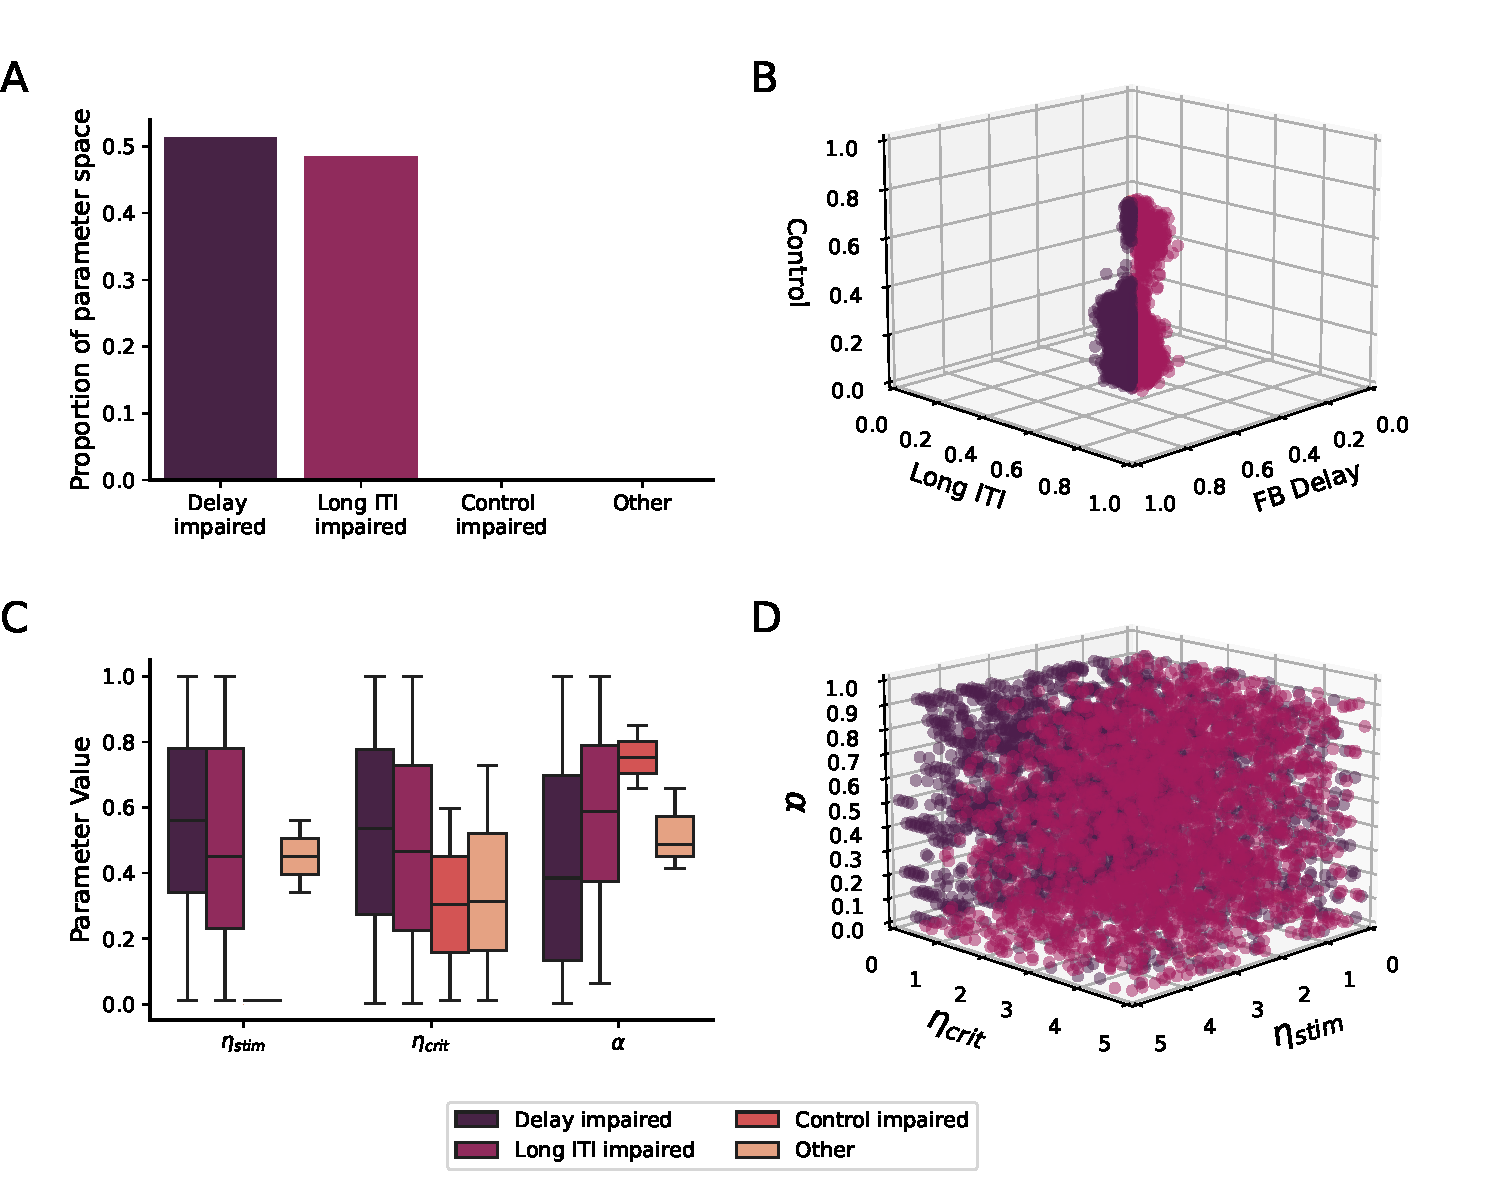
\includegraphics[width=1\textwidth]{../figures/model_working_memory.pdf}
  \caption{ 
      \textbf{A:} The proportion of parameter space where
      the time-dependent drift model predicted each of four
      qualitative patterns: (1) slower learning under
      feedback delay, (2) slower learning in the Long-ITI
      condition, (3) slower learning in the control
      condition, and (4) any other pattern. 
      % 
      \textbf{B:} Simulated trials-to-criterion for each
      condition. All scores were normalized by the largest
      trials-to-criterion value within a given parameter
      set, so all axes range from zero to one. 
      % 
      \textbf{C:} Boxplot of the parameter ranges leading to
      each PSP pattern. All parameter values were normalized
      by the largest value in the search range, so the
      ordinate ranges from zero to one for all parameters.
      % 
      \textbf{D:} Scatter plot of the parameter ranges
      associated with each PSP pattern. 
      %
      \textit{Note:} In all panels, color indicates the PSP
      pattern.
}
  \label{fig:TDD_results}
\end{figure}

Figure \ref{fig:TDD_results}A shows that the model
essentially always predicts that increasing the feedback
delay or the ITI have similar detrimental effects on
learning. The model makes this prediction because it assumes
that the criterion drifts during both the feedback delay and
during the ITI. So the critical variable for the model is
the time between the response on trial $n$ and the
presentation of the stimulus on trial $n+1$. The model
assumes that the criterion drifts during this entire time,
and therefore how this interval is divided between feedback
delay and ITI is relatively unimportant to the model
predictions. 

\subsubsection{Delay-sensitive learning model}
We simulated the performance of the delay-sensitive learning
across a wide range of parameter values for $\sigma_p$ and
$\alpha$. Specifically, in the case of $\alpha$ we stepped
through every value in the interval $[0, 1]$, with a step
size of .1. In the case of $\sigma_p$, we searched over the
interval $[0.1, 5]$, with a step size of 0.1. 

The results are shown in Figure \ref{fig:DSL_results}. Note
that virtually all combinations of the parameter values
predict that feedback delay impairs criterial learning more
than increasing the ITI. This makes sense because Equation
\ref{eq:DSL_learning} shows that the delay-sensitive
learning model predicts that increasing the feedback delay
(i.e., increasing $t_{FD}$) will impair learning -- for any
value of $\alpha>0$. Large values of $\sigma_p$ will also
impair performance because of distortion to the percept, but
this interference will be the same in all conditions.

\begin{figure}
  \centering
  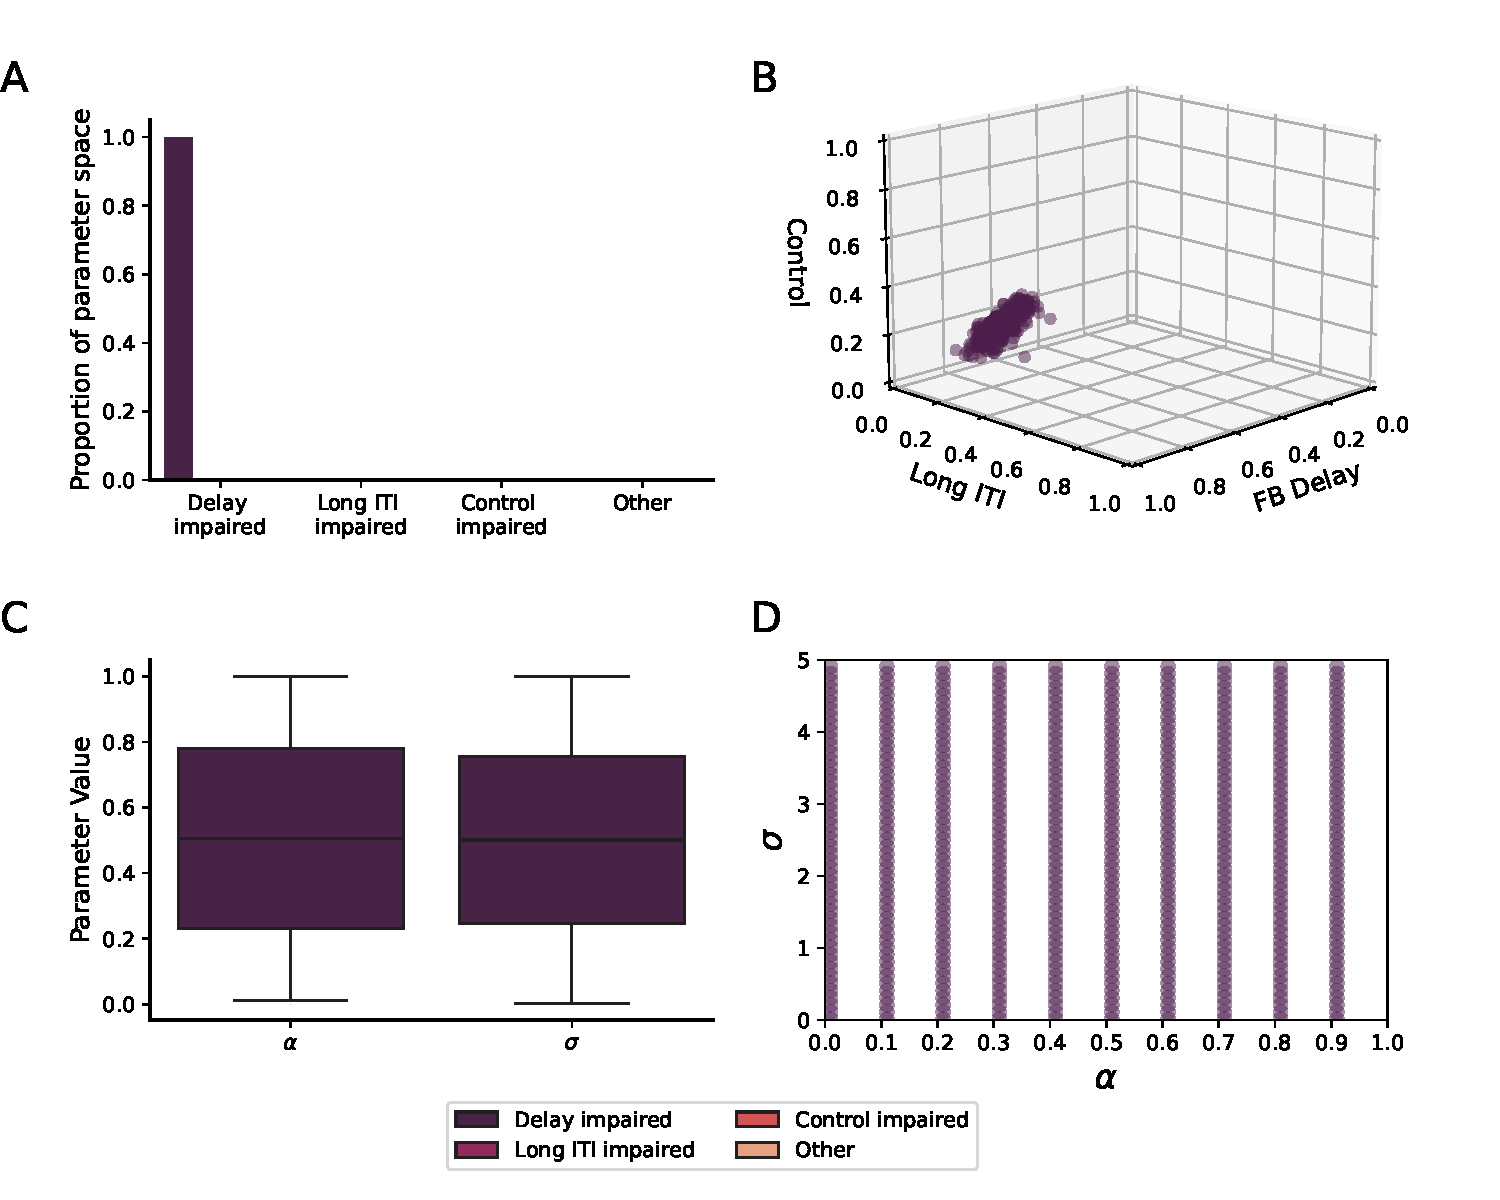
\includegraphics[width=1\textwidth]{../figures/model_procedural_supervised.pdf}
  \caption{ 
      \textbf{A:} The proportion of parameter space where
      the delay-sensitive learning model predicted each of
      four qualitative patterns: (1) slower learning under
      feedback delay, (2) slower learning in the Long-ITI
      condition, (3) slower learning in the control
      condition, and (4) any other pattern. 
      % 
      \textbf{B:} Simulated trials-to-criterion for each
      condition. All scores were normalized by the largest
      trials-to-criterion value within a given parameter
      set, so all axes range from zero to one. 
      % 
      \textbf{C:} Boxplot of the parameter ranges leading to
      each PSP pattern. All parameter values were normalized
      by the largest value in the search range, so the
      ordinate ranges from zero to one for all parameters.
      % 
      \textbf{D:} Scatter plot of the parameter ranges
      associated with each PSP pattern. 
      %
      \textit{Note:} In all panels, color indicates the PSP
      pattern.
}
  \label{fig:DSL_results}
\end{figure}

\subsubsection{Reinforcement-learning model}
We investigated the effects on performance predicted by the
reinforcement-learning model of three parameters -- the
perceptual-noise variance $\sigma^2$ and the actor and
critic learning rates (i.e., $\alpha_{actor}$ and
$\alpha_{critic}$, respectively). In the case of both
$\alpha_{actor}$ and $\alpha_{critic}$, we stepped through
every value in the interval $[0, 0.2]$, with a step size of
.01. We constrained our search over these parameters to this
interval because reinforcement-learning models are prone to
instability at very high learning rates
\parencite{SuttonBarto1998}. As evidence of this, at higher
learning rates, the model failed to learn with any
consistency -- that is, in most cases, it failed to reach
the learning criterion (12 correct responses in a row)
within the allowable 200 trials. In the case of $\sigma$, we
searched over the interval $[1, 10]$, with a step size of 1.
As with the other models, all scores were normalized by the
largest observed value.

The results are described in Figure \ref{fig:RL_results}.
Note this model predicts that delayed feedback impairs
criterial learning more than a long ITI across a wide volume
of parameters settings. As can be seen in Figure
\ref{fig:RL_results}C, the only exceptions tend to occur
when the value of any of the three parameters approaches the
maximum end of the range explored. The logic here is similar
to the delay-sensitive learning model -- that is, both
models predict that increasing the feedback delay $t_{FD}$
will impair learning -- for all values of the learning rate.

\begin{figure}
  \centering
  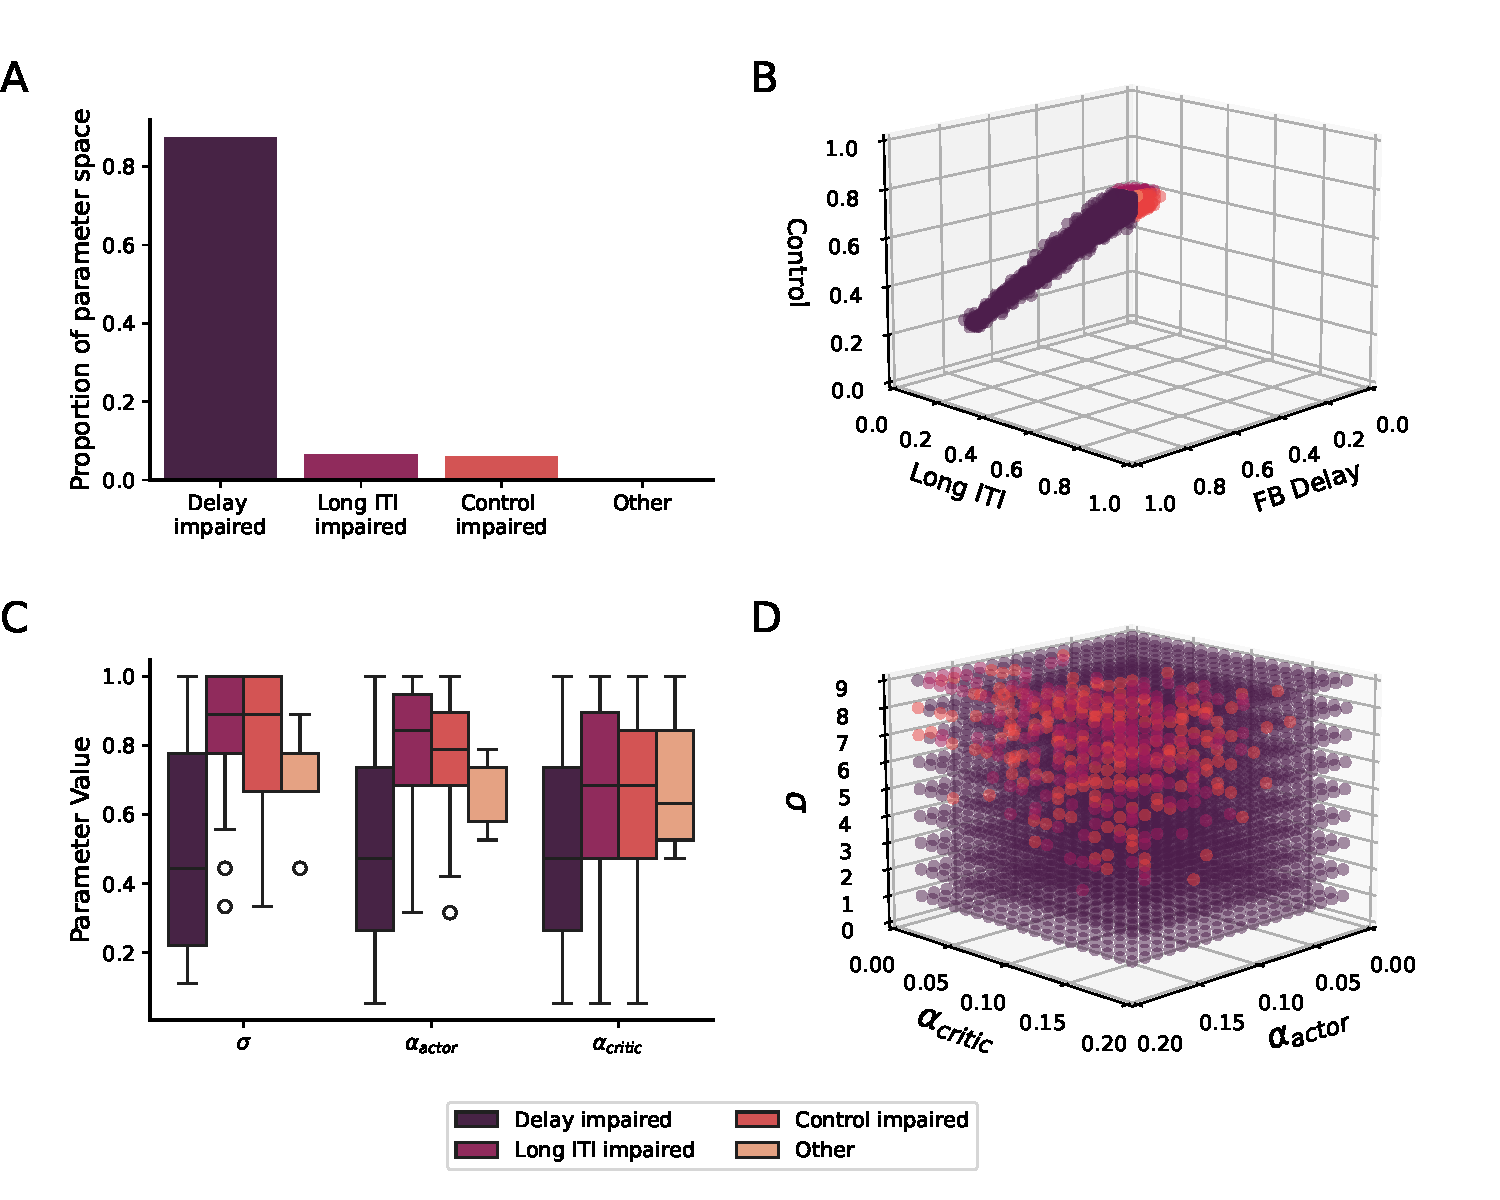
\includegraphics[width=1\textwidth]{../figures/model_procedural_reinforcement.pdf}
  \caption{ 
      \textbf{A:} The proportion of parameter space where
      the reinforcement-learning model predicted each of
      four qualitative patterns: (1) slower learning under
      feedback delay, (2) slower learning in the Long-ITI
      condition, (3) slower learning in the control
      condition, and (4) any other pattern. 
      % 
      \textbf{B:} Simulated trials-to-criterion for each
      condition. All scores were normalized by the largest
      trials-to-criterion value within a given parameter
      set, so all axes range from zero to one. 
      % 
      \textbf{C:} Boxplot of the parameter ranges leading to
      each PSP pattern. All parameter values were normalized
      by the largest value in the search range, so the
      ordinate ranges from zero to one for all parameters.
      % 
      \textbf{D:} Scatter plot of the parameter ranges
      associated with each PSP pattern. 
      %
      \textit{Note:} In all panels, color indicates the PSP
      pattern.
    }
  \label{fig:RL_results}
\end{figure}

\subsubsection{Summary of modeling results}
We investigated three criterial-learning models that make
different predictions about how increases in the feedback
delay and ITI affect learning. The time-dependent drift
model predicts that the criterion always drifts, so the
critical variable is the sum of the feedback delay and ITI.
How this sum is divided into separate feedback delay and ITI
time intervals has little effect on the model's predictions.
In contrast, the delay-sensitive learning model predicts
that feedback delays are necessarily more detrimental to
performance than increases in the ITI.  Finally, the
reinforcement-learning model also predicts that, in general,
feedback delays should impair learning more than long ITIs,
although this model is somewhat more flexible than the
delay-sensitive learning model and can account for a small
or null effect of feedback delay within a restricted region
of its parameter space. The obvious next question is how
human criterial learning is affected by these independent
variables. Experiments 2 and 3 were designed to address this
question, and therefore also to test the predictions of the
three models.

\section{Experiment 2}
Experiment 2 investigated how feedback delay and the length
of the ITI affect criterial learning in humans. As a result,
it also provides rigorous tests of the predictions of the
time-dependent drift model, the delay-sensitive learning
model, and the reinforcement-learning model.

The stimuli in Experiment 2 were circular sine-wave gratings
that varied across trials in bar width and bar orientation.
These stimuli were divided into two categories according to
their value on one of the two dimensions. In other words,
the optimal strategy was to set a response criterion on the
single relevant dimension, and then choose a categorization
response based on whether the value of the presented stimuli
on this dimension was larger or smaller than the criterion
value. 

The experiment isolated criterial learning by (1) explicitly
instructing participants on the relevant stimulus dimension
and rule structure (e.g., thick bars are ``A'', thin bars
are ``B''), and (2) eliminating variability along the
irrelevant stimulus dimension. In other words, the
instructions identified the relevant stimulus dimension, and
as a result, the only learning required was criterial
learning. 

\subsection{Method}

\subsubsection{Apparatus}
All experiments were performed in a dimly lit room.
Participants sat approximately 24'' from a 17'' $\times$
11'' monitor running at a resolution of 1680 $\times$ 1050
pixels. Participants made category judgments by pressing the
`d' or `k' keys on a standard computer keyboard for `A' or
`B' choices, respectively. Stickers with bold print `A' or
`B' were placed on the appropriate keys.

\subsubsection{Stimuli and Categories}
Stimuli were circular sine-wave gratings that varied in bar
width and bar orientation, drawn from various 1-dimensional
uniform distributions specific to the current category
problem. We first defined an arbitrary 2-dimensional
$[0-100,0-100]$ stimulus space, and then split each
dimension of this space into 7 bins of width 14 units each.
Each $(x,y)$ pair from this arbitrary stimulus space was
converted to a grating according to the nonlinear
transformations defined by
\textcite{treutwein1989perceptual}, which roughly equate the
salience of each dimension (for details, see also
\textcite{CrossleyAshby2015}).

The structure of the various criterial-learning tasks is
illustrated in Figure \ref{fig_design_exp_1_space}. Each
criterial-learning problem was created by first randomly
selecting a relevant dimension, and then randomly selecting
one of the 7 bins defined on that dimension. Each bin was
also associated with a corresponding unique value on the
irrelevant dimension. We buffered the to-be-learned response
criterion by 10\% of total bin width on either side with a
no-stimulus region. Random uniform samples from the
remaining eligible region of each bin were then selected and
presented to the participant until 9 correct responses out
of any 10 responses in a row advanced the participant to the
next problem. Note that every category problem was a simple
one-dimensional rule in which optimal accuracy was 100\%.
Note also that the relative location of the optimal response
criterion varied across problems.

\begin{figure}
  \centering
  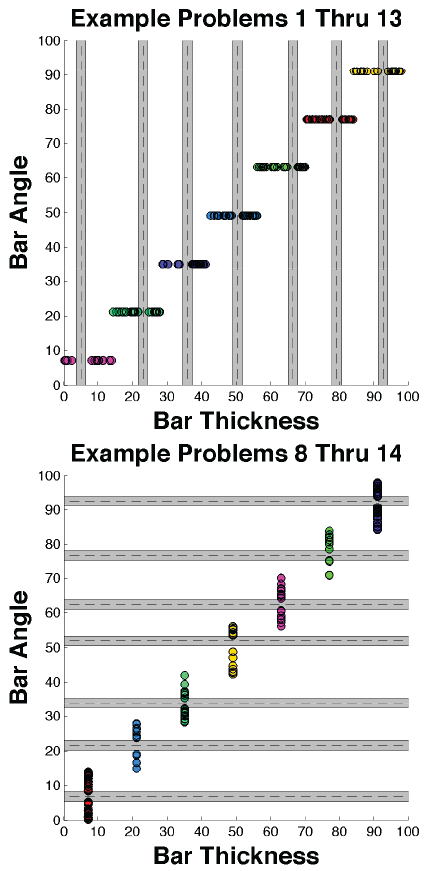
\includegraphics[width=.5\textwidth]{../figures/fig_design_exp_1_space.png}
  \caption{
      Category sample space. Different colors represent
      different category problems. Dashed lines are category
      boundaries (criterion) and the surrounding solid lines
      mark the no-stimulus region in which no stimuli were
      sampled.
}
  \label{fig_design_exp_1_space}
\end{figure}

\subsubsection{Procedure}
There were three conditions (described in detail in Table
\ref{conditions_exp_1}). In the Delayed-Feedback condition,
feedback was delayed 3.5 s after the response and the ITI
was 0.5 s. In the Long-ITI condition, feedback was delayed
0.5 s after the response and the ITI was 3.5 s. Finally, in
the Control condition, feedback was delayed 0.5 s after the
response and the ITI was 0.5 s.

Each participant completed a series of one-dimensional
category-learning tasks or problems, which are described in
Figure \ref{fig_design_exp_1_space}. Each problem included
stimuli in two distinct clusters that varied over a
restricted range of the relevant dimension. Critically, the
optimal criterion value varied from problem-to-problem with
respect to its position within this range. For example, for
some problems the optimal criterion was below the midpoint
of the range and for other problems it was above the
midpoint. 

Participants were explicitly told the relevant dimension for
each problem, as well as the generic response mapping (e.g.,
thick bars = ``A'', thin bars = ``B''). Figure
\ref{fig:trial} shows the structure of an example trial,
along with an example of a typical category structure. All
trials in every condition included a 500 ms fixation cross,
a response-terminated stimulus, a circular white-noise mask,
corrective feedback, and an inter-trial interval (ITI) that
varied according to condition. The text `Correct' was
displayed in centered, large green font after correct
responses, and the text `Incorrect' was displayed in
centered, large red font after incorrect responses.

Participants practiced each problem until they responded
correctly on 9 of the previous 10 trials. At this point, the
problem changed. Each participant completed as many problems
as possible in 512 trials or until they had been in the lab
for 60 minutes (including time to acquire consent and give
instructions), at which point the session was terminated.

\begin{figure}
  \centering
  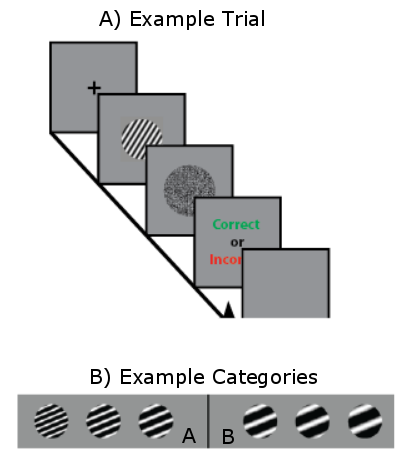
\includegraphics[width=.5\textwidth]{../figures/fig_design_exp_1.png}
  \caption{
      Example trial and category problem. A) Events that
      occurred on each trial. B) An example of a typical
      category structure.
}
  \label{fig:trial}
\end{figure}

\begin{table}
    \caption{
        Durations (in s) of Trial Events in each Condition.
    }
    \label{conditions_exp_1}
    \begin{tabular}{c|cccc}
        Conditions & Stim & Mask & FB & ITI \\[0.5ex] \hline Control & RT & 0.5 &
        1.0 & 0.5 \\[0.5ex]
        \\[-1.5ex] Delayed Feedback &
        RT & 3.5 & 1.0 & 0.5 \\[0.5ex]   Long ITI & RT & 0.5 & 1.0 & 3.5
        \\[0.5ex]
    \end{tabular}
\end{table}

\subsubsection{Participants}
Fifty-nine participants participated in Experiment 2. All
were UCSB undergraduates and received course credit for
their participation. All had normal or corrected to normal
vision. We randomly assigned each participant to one of
three conditions (target $N>16$ per condition based on
similar previous research): Delayed Feedback ($N = 20$);
Long ITI ($N = 21$), Control ($ N = 17$).

\subsection{Results}
Figure \ref{fig_gmm_hist_1} shows a relative frequency
histogram of the trials-to-criterion observed across all
three conditions. The histogram shows that the majority of
participants were able to learn each problem on average in
less than 100 trials. However, this histogram also shows
that a subset of participants required many more trials to
learn each problem. Given that each problem is very simple
and that the relevant dimension of each problem is
explicitly instructed to participants, it is likely that the
participants in the tails of this distribution did not pay
attention to the instructions, were not motivated to learn
the task, were distracted by other factors, or should be
considered outliers for some other reason. 

\begin{figure}
  \centering
  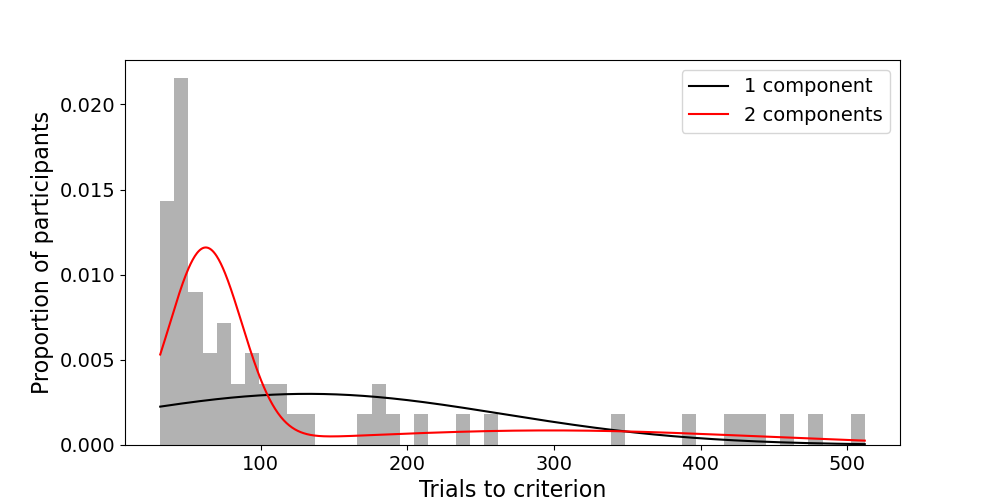
\includegraphics[width=.8\textwidth]{../figures/fig_exp_1_gmm.png}
  \caption{
      Relative frequency histogram of the
      trials-to-criterion observed across all three
      conditions in Experiment 2. The black line are the
      predictions of the best-fitting one-component Gaussian
      Mixture Model to these data, whereas the red line
      represents the best fit of the two-component Gaussian
      Mixture Model. The two-component model provided a
      significantly better fit according to AIC, BIC, and a
      likelihood ratio test.
}
  \label{fig_gmm_hist_1}
\end{figure}

% AIC for 1 component: 735.7652217198266
% AIC for 2 components: 662.8095009936025
% 
% BIC for 1 component: 739.8861077409194
% BIC for 2 components: 673.1117160463345
%
% LRT statistic: 78.95572072622417
% Degrees of freedom: 3
% P-value: 5.140608761896481e-17

We modeled the distribution shown in Figure
\ref{fig_gmm_hist_1} using a Gaussian mixture model with two
components. The first component captured participants with a
relatively low mean number of trials-to-criterion, while the
second component identified outliers according to the above
rationale. We compared the fit of this two-component model
to a single-component model using the Akaike Information
Criterion (AIC) and Bayesian Information Criterion (BIC),
both of which indicated a better fit for the two-component
model (AIC: 662.81 vs. 735.77; BIC: 673.11 vs. 739.89).
Additionally, a likelihood ratio test confirmed that the
two-component model provided a significantly better fit than
the one-component model ($\chi^2(3) = 78.96$, $p < .001$).
Outlier participants were then excluded from further
analysis.  After making these exlcusions, we were left with
the following sample sizes: Control condition ($ N = 11$);
Delayed-Feedback condition ($N = 14$);  Long-ITI condition
($N = 17$).

Figure \ref{fig_exp_1_t2c}A shows the mean
trials-to-criterion in each condition of Experiment 2.  A
one-way ANOVA revealed a significant effect of condition
($F(2, 39) = 6.17$, $p < .01$, $\eta^2 = .24$) and planned
comparisons revealed that performance in the
Delayed-Feedback condition was significantly worse than in
either the Control condition ($t(23.00) = 2.70$, $p < .05$)
or the Long-ITI condition ($t(20.96) = 2.94$, $p < .01$).
Performance in the Control and Long-ITI conditions did not
differ significantly from each other ($t(17.99) = 0.22$, $p
= .83$).

%   Source  ddof1  ddof2         F     p-unc       np2
% 0    cnd      2     39  6.171331  0.004693  0.240398
%
%           A          B         T        dof     p-unc
% 0     Delay   Long ITI  2.938217  20.959026  0.007864
% 1     Delay  Short ITI  2.701083  22.997274  0.012748
% 2  Long ITI  Short ITI  0.219862  17.987044  0.828454

Figure \ref{fig_exp_1_t2c}B shows the mean number of
problems solved in each condition of Experiment 2. A one-way
ANOVA revealed a significant effect of condition ($F(2, 39)
= 5.77$, $p < .01$, $\eta^2 = .23$). Planned comparisons
revealed that performance in the Delayed-Feedback condition
was significantly worse than in the Control condition
($t(18.54) = -3.28$, $p < .01$) and worse than in the Long
ITI condition ($t(21.60) = -2.14$, $p < .05$).  Performance
in the Control and Long-ITI conditions did not differ
significantly from each other ($t(25.97) = -1.50$, $p=.15$).

%   Source  ddof1  ddof2         F     p-unc       np2
% 0    cnd      2     39  5.766358  0.006399  0.228223
% 
%           A          B         T        dof     p-unc
% 0     Delay   Long ITI -2.143777  21.590392  0.043579
% 1     Delay  Short ITI -3.277500  18.536603  0.004061
% 2  Long ITI  Short ITI -1.501591  25.965920  0.145267

\begin{figure}
  \centering
  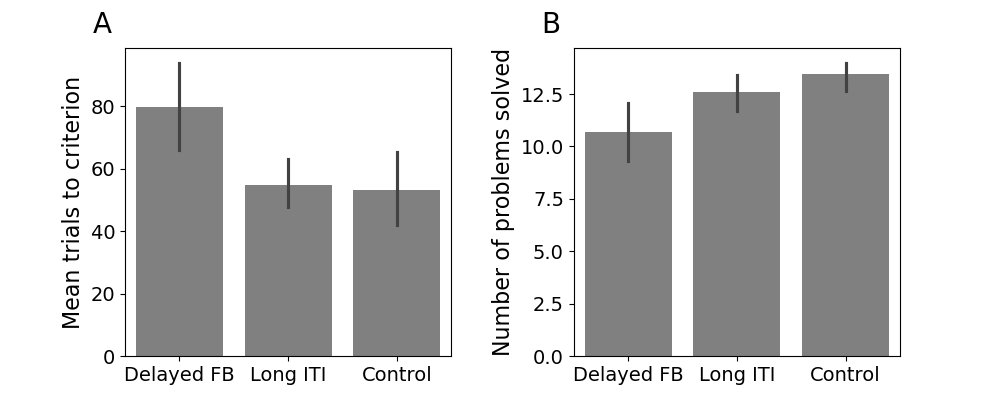
\includegraphics[width=.8\textwidth]{../figures/fig_exp_1_t2c.png}
    \caption{
        \textbf{A}: Mean trials to criterion in each
        condition of Experiment 2. Error bars are standard
        errors of the mean.
        %
        \textbf{B}: Mean number of problems solved in each
        condition of Experiment 2. Error bars are standard
        errors of the mean.
}
  \label{fig_exp_1_t2c}
\end{figure}

\section{Experiment 3}
Experiment 3 was designed to reinforce the findings of
Experiment 2 by using the same design but with stimuli that
have binary-valued dimensions, thereby eliminating criterial
learning. Unlike Experiment 2, we did not explicitly
instruct participants on the relevant stimulus dimension in
Experiment 3.  While Experiment 2 isolated criterial
learning from rule selection and rule switching, this
experiment isolates rule selection and switching from
criterial learning. Therefore, Experiment 3 was designed to
test whether the impaired learning that we observed in
Experiment 2 when the feedback was delayed can be attributed
principally to criterial learning or whether it could be due
to some more general category-learning process.

\subsection{Method}

\subsubsection{Apparatus}
The apparatus was the same as in Experiment 2.

\subsubsection{Stimuli and Categories}
The stimuli consisted of colored geometric figures presented
on a colored background. These varied across six binary
dimensions: the number of items (either one or two), the
size of the items (small or large), the color of the items
(yellow or blue), the shape of the items (circle or square),
the texture of the background (smooth or rough), and the
orientation of the background (horizontal or tilted by 20
degrees). This combination resulted in a total of 64 unique
stimuli ($2^6$). An example trial and stimuli are shown in
Figure \ref{fig_design_exp_2}. In all conditions, the order
of stimulus presentation was fully randomized for each
participant, and the relevant dimension for each problem was
selected randomly without replacement from the set of six
dimensions.

\begin{figure}
  \centering
  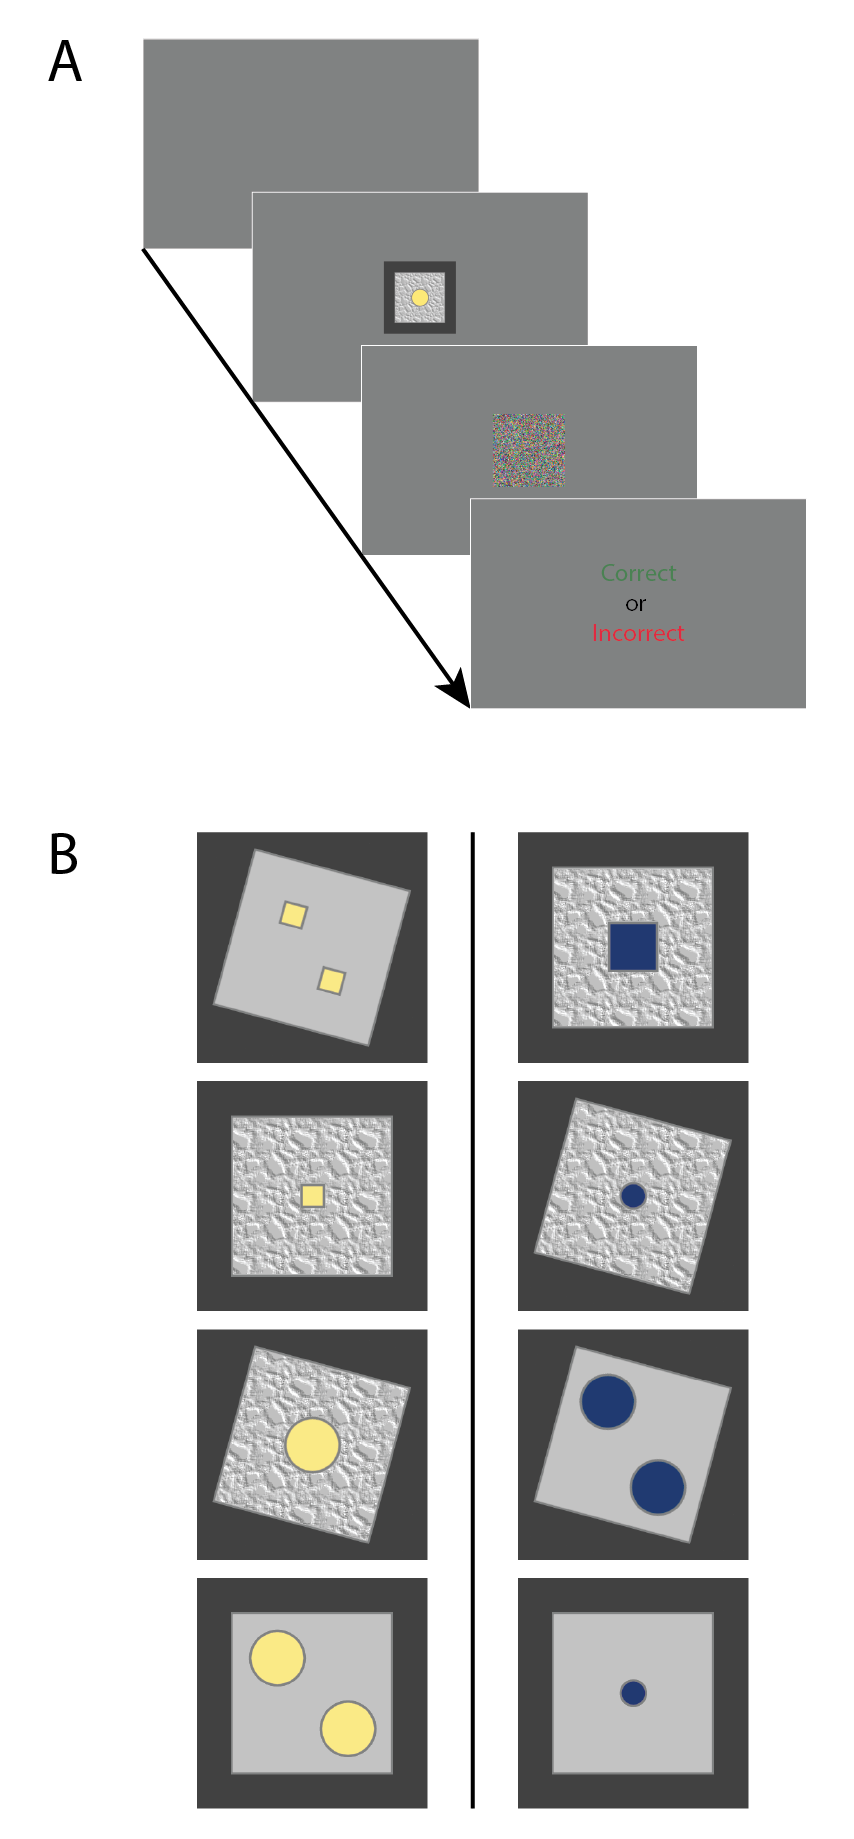
\includegraphics[width=.5\textwidth]{../figures/fig_design_exp_2.png}
  \caption{
      \textbf{A:} An example trial from Experiment 3.
      \textbf{B:} Eight example stimuli (out of 64 total
      stimuli) from a possible one-dimensional rule problem.
      In this case the correct rule is `A' if the shape
      color is yellow and `B' if the shape color is blue.
      The solid line represents the category boundary.
}
  \label{fig_design_exp_2}
\end{figure}

\subsubsection{Procedure}
Participants received detailed instructions about the task.
However, unlike in Experiment 2, they were not informed of
the relevant dimension or the correct rule. The trial timing
for the Delayed-Feedback and Long-ITI conditions in
Experiment 3 were the same as in Experiment 2. Experiment 3
did not include a condition that was analogous to the
Control condition of Experiment 2. Participants practiced
each problem until they responded correctly on 12
consecutive trials. At this point, the problem changed. Each
participant completed as many problems as possible in 600
trials or until they had been in the lab for 30 minutes
(including time to acquire consent and give instructions),
at which point the session was terminated.

\subsubsection{Participants}
Thirty-four participants participated in Experiment 3. All
were Macquarie University undergraduates and received course
credit for their participation. All had normal or corrected
to normal vision. We randomly assigned each participant to
one of two conditions: Delayed Feedback ($N = 17$) or Long
ITI ($N = 17$).

\subsection{Results}
Figure \ref{fig_gmm_hist_2} shows a relative frequency
histogram of the trials-to-criterion observed in both
conditions. The histogram shows that the majority of
participants were able to learn each problem on average in
less than 100 trials.  Unlike Experiment 2, there were no
highly suspicious outliers in this data set. Nevertheless,
for symmetry with Experiment 2, we performed the same
Gaussian mixture model analysis as used there. The
two-component model provided a slightly smaller AIC value
(317.40 vs. 317.78), but a slightly larger BIC value (325.03
vs. 320.83). The likelihood-ratio test was not significant
($\chi^2(3) = 6.38$, $p = .09$). We therefore did not
exclude any participants from further analysis in Experiment
2.

\begin{figure}
  \centering
  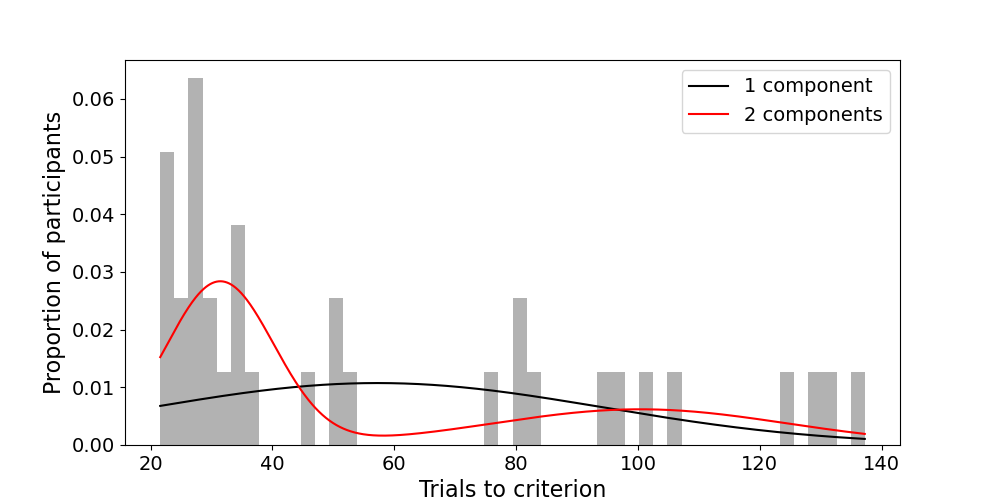
\includegraphics[width=.8\textwidth]{../figures/fig_exp_2_gmm.png}
  \caption{
      Relative frequency histogram of the
      trials-to-criterion observed across all three
      conditions in Experiment 3. The black line represents
      the best fit of the one-component Gaussian Mixture
      Model, and the red line represents the best fit of the
      two-component Gaussian Mixture Model.
}
  \label{fig_gmm_hist_2}
\end{figure}

% AIC for 1 component: 317.77535652645616
% AIC for 2 components: 317.3995958509652
% 
% BIC for 1 component: 320.8280775756885
% BIC for 2 components: 325.03139847404606
% 
% LRT statistic: 6.3757606754909375
% Degrees of freedom: 3
% P-value: 0.09469309595624516

Figure \ref{fig_exp_2_t2c}A shows the mean
trials-to-criterion in each condition of Experiment 3. An
independent-samples t-test revealed no significant effect of
condition ($t(32.0)=0.69$, $p = .50$, $\eta^2 = .01$).  The
mean number of problems solved by each participant is shown
in Figure \ref{fig_exp_2_t2c}B. An independent-samples
t-test revealed no significant effect of condition ($t(32) =
-0.49$, $p = .63$, $\eta^2 = .01$).

%   Source  ddof1  ddof2        F     p-unc       np2
% 0    cnd      1     32  0.47046  0.497715  0.014489
% 
%        A          B         T   dof     p-unc
% 0  delay  immediate  0.685901  32.0  0.497715

%   Source  ddof1  ddof2         F    p-unc       np2
% 0    cnd      1     32  0.235294  0.63093  0.007299
% 
%        A          B         T   dof    p-unc
% 0  delay  immediate -0.485071  32.0  0.63093

\begin{figure}
  \centering
  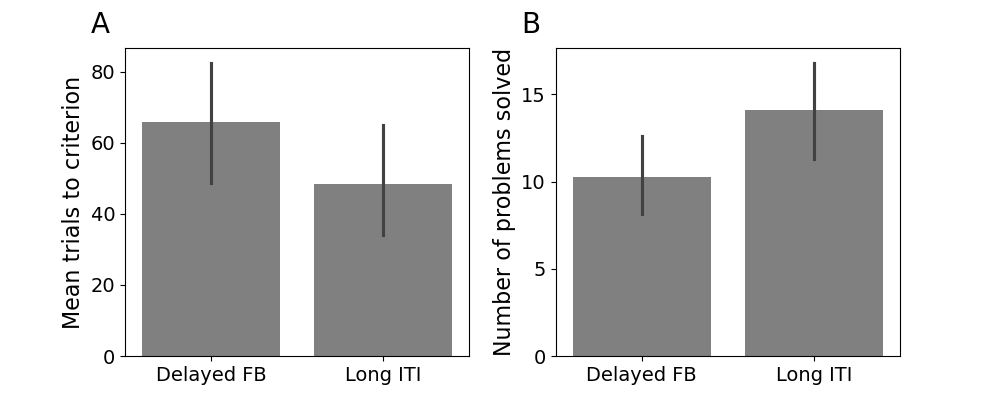
\includegraphics[width=.8\textwidth]{../figures/fig_exp_2_t2c.png}
    \caption{
        \textbf{A}: Mean trials to criterion in each
        condition of Experiment 3. Error bars are standard
        errors of the mean.
        %
        \textbf{B}: Mean number of problems solved in each
        condition of Experiment 3. Error bars are standard
        errors of the mean.
}
  \label{fig_exp_2_t2c}
\end{figure}

\subsection{Discussion of Experiments 2 and 3}
Experiment 2 clearly showed that a short feedback delay of
3.5 s slowed criterial learning. In contrast, increasing the
ITI to this same value had no effect on learning. The task
we used was one-dimensional category learning, but we
isolated criterial learning by instructing participants
about the optimal strategy. Specifically, we told them which
stimulus dimension was relevant and that there was no
trial-by-trial variability on the irrelevant dimension.
Although these results strongly suggest that the feedback
delay had its interfering effects on criterial learning,
Experiment 3 was designed to confirm this inference. The
goal here was to examine the effects of the same feedback
delays and ITIs on performance in a one-dimensional
category-learning task that did not require any criterial
learning, but did require category-learning processes that
are thought to mediate rule discovery (e.g., rule selection
and switching). If the feedback delay effects observed in
Experiment 2 were acting on some general category-learning
skill then we should have seen the same interfering effects
of feedback delay in Experiment 3. However, if the
feedback-delay interference of Experiment 2 was operating
selectively on criterial learning, then it should disappear
in Experiment 3, since no criterial learning was required.
Our results strongly supported this latter prediction.
Therefore, Experiments 2 and 3 together strongly suggest
that criterial learning is impaired by feedback delays and
is relatively unaffected by the length of the ITI.

Two prior studies investigated similar issues. First, Ell
and colleagues reported that feedback delay and also a
concurrent memory-scanning task each impaired rule-based
category learning \parencite{ell2009critrial}. Based on
these results, they hypothesized that criterial learning may
be tied to working-memory capacity and therefore to explicit
cognitive mechanisms. However, criterial learning was
confounded with rule selection and task difficulty in their
design.  Furthermore, \textcite{ell2009critrial} found that
feedback delay only impaired learning when working memory
demand was high -- that is, when participants had to learn
more than one response criterion for optimal performance. In
contrast, we found that feedback delay impairs learning even
when working memory demands are trivial (participants never
have to keep in mind more than one criterion).

Second, \textcite{bohil2014implicit} reported that the
effects of unequal base rates on criterion placement in
rule-based category learning were diminished under delayed
feedback and also under an observational training protocol
that is also thought to selectively impair basal
ganglia-dependent associative-learning mechanisms. These
results are consistent with our findings. However, because
they were obtained by manipulating base rates, it is
difficult to conclude that the delay affected criterial
learning, \emph{per se}. For example, consider a simple
two-stage model in which the first stage learns the base
rates and the second stage uses what the first stage learned
to adjust the response criterion appropriately. The
\textcite{bohil2014implicit} results are also consistent
with the hypothesis that the feedback delay impaired the
first of these stages but not the second. Our results
strongly suggest that feedback delays impair criterial
learning (and therefore the second of these hypothetical
stages).

\section{General Discussion}
We developed three novel models of criterial learning that
were designed to explore how feedback delay and ITI duration
affect criterial learning. Two of these models assumed that
decisions are made by comparing the current percept to a
stored referent, or criterion, and that the remembered value
of this criterion is updated following error feedback via a
gradient-descent learning rule. The first of these models,
the time-dependent drift model, posits that both the
criterion and the percept drift over time, leading to
similar impairments when feedback is delayed or the ITI is
increased. The second model, the delay-sensitive learning
model, assumes that although neither the percept nor the
criterion drift over time, optimal criterial learning
requires immediate feedback. As a result, this model
predicts that increasing the feedback delay will slow the
rate of criterial learning. The third model, the
reinforcement-learning model, assumes that criterial
learning arises through the gradual formation of
stimulus-response associations, rather than via the
construction of a response criterion. This model also
assumes that the rate at which these associations are
learned is slowed by feedback delays.

Simulations of these models in a task that was structurally
identical to Experiment 2 revealed that the time-dependent
drift model typically predicts that the most important
variable for criterial learning is the total amount of time
between the response and the stimulus presentation that
defines the next trial. Where the feedback is presented
within this interval is relatively unimportant. In contrast,
both the delay-sensitive learning model and the
reinforcement-learning model consistently predict that
feedback delays should impair performance more than a long
ITI. 

The experiments were designed to test these predictions. Our
results strongly suggested that human criterial learning is
sensitive to feedback delay but not to the ITI duration.
This suggests that the delay-sensitive learning model and
the reinforcement-learning model provide a better account of
human behavior across wide ranges of their respective
parameter spaces than the time-dependent drift model.

The time-dependent drift model was based on the idea that
criterial learning might be entirely supported by working
memory. The assumption of drift in this model stems from the
understanding that maintaining items in working memory is
inherently challenging.  The longer an item is held, the
more likely it is to deteriorate. Therefore, the model
predicts that performance should deteriorate as the time
between the response on trial $n$ and stimulus presentation
on trial $n+1$ increases, regardless of how this interval is
divided between feedback delay and ITI. The results of
Experiments 1 and 2 strongly disconfirm this prediction. 

In contrast, the delay-sensitive learning model was inspired
by the idea that a response criterion might be encoded in a
more stable memory system. One appealing candidate for this
function is the cerebellum, where synaptic plasticity has
been shown to follow a gradient descent learning rule and
also to be sensitive to feedback timing
\parencite{brudner2016delayed, held_adaptation_1966,
honda_adaptation_2012, kitazawa_effects_1995,
kitazawa_prism_2002}.  Finally, the reinforcement-learning
model draws on the idea that criterial learning could emerge
through stimulus-response association learning driven by
dopamine-dependent synaptic plasticity in the striatum. This
process aligns with established theories of category
learning that posit a key role to this learning process in
the basal ganglia \cite{AshbyCOVIS1998}.

Our results do not strongly favor the delay-sensitive
learning model over the reinforcement learning model or vice
versa. The critical disagreement between these accounts is
whether the criterion has any real psychological meaning. In
the delay-sensitive learning model it does, and thus this
model is psychologically similar to the time-dependent drift
model -- the main disagreement being about whether the
representation of the criterion is stable and if the
updating of the criterion is sensitive to feedback delay.

The reinforcement-learning model makes very different
psychological assumptions. This model assumes that behaviors
described as ``criterial learning'' are actually mediated by
the learning of stimulus-response associations. According to
this account, the criterion has no internal representation
and therefore no psychological meaning. Testing between
these two very different accounts of criterial learning
should be a focus of future research. 

We are not aware of any data that directly addresses the
question of whether a response criterion is a fundamental
psychological construct, as the delay-sensitive learning
model suggests, or whether it is unnecessary, as assumed by
the reinforcement learning model. Even so, there are some
results in the category-learning literature that support the
interpretation of the reinforcement-learning model. In
information-integration (II) category-learning tasks, the
optimal strategy is similarity-based, and difficult or
impossible to describe verbally
\parencite[e.g.,][]{AshbyValentin2018}. When the stimuli
vary on two dimensions, the stimuli from contrasting
categories can be partitioned by a decision bound that is
conceptually similar to a response criterion. In both cases,
all stimuli on one side are associated with one response,
and all stimuli on the other side are associated with the
contrasting response. Furthermore, in agreement with
Experiment 2, II category learning is impaired by short
feedback delays \parencite{MaddoxAshbyBohil2003,
MaddoxIng2005}. The analogous question in II category
learning is whether the decision bound is learned directly
or whether it is simply the set of points that divide the
perceptual space into contrasting response regions.  In
fact, the evidence strongly supports this latter
interpretation \parencite{AshbyWaldron1999, CasaleEtAl2012}.
For example, if the decision bound is learned, then it
should be possible to apply this bound to novel stimuli.
With rule-based categories, this is easy for participants,
but with II categories there is no evidence that the
response strategy that participants learn can be generalized
to novel stimuli \parencite{CasaleEtAl2012} -- a result that
strongly supports the hypothesis that the decision bound has
no psychological meaning. 

Our results clearly demonstrate that criterial learning is
impaired by delayed feedback, and not by extending the
intertrial interval. These results are consistent with the
hypothesis that criterial learning is a form of
basal-ganglia mediated associative learning, and are
inconsistent with hypotheses that criterial learning is a
working-memory-based process. Thus, our results provide a
critical constraint on future models of rule-based
classification and decision making, and possibly also on
more general accounts of criterion setting, such as in
signal detection theory.

Previous studies have failed to find that feedback delays
impair rule-based category learning, and on the face of it,
this seems to contradict our finding that feedback delays
impair criterial learning. However, all earlier RB studies
that looked for effects of a feedback delay, either used
binary-valued stimulus dimension and so no criterial
learning was needed, or else set the response criterion
exactly midway between the category prototypes, which makes
criterial learning trivial. For example, under these
conditions, criterial learning might not even require
feedback. The unsupervised category-learning experiments
reported by \textcite{ashby1999dominance} provide strong
support for this because all of their rule-based
participants learned the correct criterion (which was midway
between the category means), even though the task was
completely unsupervised. Moreover, all previous studies
failed to isolate criterial learning, so even if there was
an effect of feedback delay on criterial learning, it could
have been masked by larger effects caused by other
rule-learning processes.

Criterial learning is among the most classic and ubiquitous
of all cognitive skills. For example, signal-detection
theory teaches that it is the central form of learning in an
enormous range of decision-making tasks -- everything from
simple YES-NO detection of a weak signal to assessing the
guilt or innocence of a defendant in a jury trial. Our
results suggest that even in simple rule-based tasks,
criterial learning seems to be subserved, at least in part,
by associative mechanisms. Most current theories tend to
classify tasks as either executive function (e.g.,
rule-based category learning) or procedural (e.g., mirror
tracing). Our results suggest that such classification
schemes might oversimplify how humans perform these tasks,
and therefore that much more work is needed to understand
how different learning and memory systems interact.

% TODO
\section{Transparency and Openness}
All data have been made publicly available at the [trusted
repository name] and can be accessed at [persistent URL or
DOI].

\section{Author Notes}
Preparation of this article was supported by Public Health
Service Grant MH2R01-063760.

\printbibliography

\end{document}
